% Options for packages loaded elsewhere
\PassOptionsToPackage{unicode}{hyperref}
\PassOptionsToPackage{hyphens}{url}
\PassOptionsToPackage{dvipsnames,svgnames,x11names}{xcolor}
%
\documentclass[
  letterpaper,
  DIV=11,
  numbers=noendperiod]{scrreprt}
\usepackage{amsmath,amssymb}
\usepackage{lmodern}
\usepackage{iftex}
\ifPDFTeX
  \usepackage[T1]{fontenc}
  \usepackage[utf8]{inputenc}
  \usepackage{textcomp} % provide euro and other symbols
\else % if luatex or xetex
  \usepackage{unicode-math}
  \defaultfontfeatures{Scale=MatchLowercase}
  \defaultfontfeatures[\rmfamily]{Ligatures=TeX,Scale=1}
\fi
% Use upquote if available, for straight quotes in verbatim environments
\IfFileExists{upquote.sty}{\usepackage{upquote}}{}
\IfFileExists{microtype.sty}{% use microtype if available
  \usepackage[]{microtype}
  \UseMicrotypeSet[protrusion]{basicmath} % disable protrusion for tt fonts
}{}
\makeatletter
\@ifundefined{KOMAClassName}{% if non-KOMA class
  \IfFileExists{parskip.sty}{%
    \usepackage{parskip}
  }{% else
    \setlength{\parindent}{0pt}
    \setlength{\parskip}{6pt plus 2pt minus 1pt}}
}{% if KOMA class
  \KOMAoptions{parskip=half}}
\makeatother
\usepackage{xcolor}
\IfFileExists{xurl.sty}{\usepackage{xurl}}{} % add URL line breaks if available
\IfFileExists{bookmark.sty}{\usepackage{bookmark}}{\usepackage{hyperref}}
\hypersetup{
  pdftitle={Example Jupyter Notebook},
  colorlinks=true,
  linkcolor={blue},
  filecolor={Maroon},
  citecolor={Blue},
  urlcolor={Blue},
  pdfcreator={LaTeX via pandoc}}
\urlstyle{same} % disable monospaced font for URLs
\usepackage{color}
\usepackage{fancyvrb}
\newcommand{\VerbBar}{|}
\newcommand{\VERB}{\Verb[commandchars=\\\{\}]}
\DefineVerbatimEnvironment{Highlighting}{Verbatim}{commandchars=\\\{\}}
% Add ',fontsize=\small' for more characters per line
\usepackage{framed}
\definecolor{shadecolor}{RGB}{241,243,245}
\newenvironment{Shaded}{\begin{snugshade}}{\end{snugshade}}
\newcommand{\AlertTok}[1]{\textcolor[rgb]{0.68,0.00,0.00}{#1}}
\newcommand{\AnnotationTok}[1]{\textcolor[rgb]{0.37,0.37,0.37}{#1}}
\newcommand{\AttributeTok}[1]{\textcolor[rgb]{0.40,0.46,0.14}{#1}}
\newcommand{\BaseNTok}[1]{\textcolor[rgb]{0.68,0.00,0.00}{#1}}
\newcommand{\BuiltInTok}[1]{\textcolor[rgb]{0.00,0.46,0.62}{#1}}
\newcommand{\CharTok}[1]{\textcolor[rgb]{0.13,0.47,0.30}{#1}}
\newcommand{\CommentTok}[1]{\textcolor[rgb]{0.37,0.37,0.37}{#1}}
\newcommand{\CommentVarTok}[1]{\textcolor[rgb]{0.37,0.37,0.37}{\textit{#1}}}
\newcommand{\ConstantTok}[1]{\textcolor[rgb]{0.56,0.35,0.01}{#1}}
\newcommand{\ControlFlowTok}[1]{\textcolor[rgb]{0.00,0.46,0.62}{#1}}
\newcommand{\DataTypeTok}[1]{\textcolor[rgb]{0.68,0.00,0.00}{#1}}
\newcommand{\DecValTok}[1]{\textcolor[rgb]{0.68,0.00,0.00}{#1}}
\newcommand{\DocumentationTok}[1]{\textcolor[rgb]{0.37,0.37,0.37}{\textit{#1}}}
\newcommand{\ErrorTok}[1]{\textcolor[rgb]{0.68,0.00,0.00}{#1}}
\newcommand{\ExtensionTok}[1]{\textcolor[rgb]{0.00,0.46,0.62}{#1}}
\newcommand{\FloatTok}[1]{\textcolor[rgb]{0.68,0.00,0.00}{#1}}
\newcommand{\FunctionTok}[1]{\textcolor[rgb]{0.28,0.35,0.67}{#1}}
\newcommand{\ImportTok}[1]{\textcolor[rgb]{0.00,0.46,0.62}{#1}}
\newcommand{\InformationTok}[1]{\textcolor[rgb]{0.37,0.37,0.37}{#1}}
\newcommand{\KeywordTok}[1]{\textcolor[rgb]{0.00,0.46,0.62}{#1}}
\newcommand{\NormalTok}[1]{\textcolor[rgb]{0.00,0.46,0.62}{#1}}
\newcommand{\OperatorTok}[1]{\textcolor[rgb]{0.37,0.37,0.37}{#1}}
\newcommand{\OtherTok}[1]{\textcolor[rgb]{0.00,0.46,0.62}{#1}}
\newcommand{\PreprocessorTok}[1]{\textcolor[rgb]{0.68,0.00,0.00}{#1}}
\newcommand{\RegionMarkerTok}[1]{\textcolor[rgb]{0.00,0.46,0.62}{#1}}
\newcommand{\SpecialCharTok}[1]{\textcolor[rgb]{0.37,0.37,0.37}{#1}}
\newcommand{\SpecialStringTok}[1]{\textcolor[rgb]{0.13,0.47,0.30}{#1}}
\newcommand{\StringTok}[1]{\textcolor[rgb]{0.13,0.47,0.30}{#1}}
\newcommand{\VariableTok}[1]{\textcolor[rgb]{0.07,0.07,0.07}{#1}}
\newcommand{\VerbatimStringTok}[1]{\textcolor[rgb]{0.13,0.47,0.30}{#1}}
\newcommand{\WarningTok}[1]{\textcolor[rgb]{0.37,0.37,0.37}{\textit{#1}}}
\usepackage{longtable,booktabs,array}
\usepackage{calc} % for calculating minipage widths
% Correct order of tables after \paragraph or \subparagraph
\usepackage{etoolbox}
\makeatletter
\patchcmd\longtable{\par}{\if@noskipsec\mbox{}\fi\par}{}{}
\makeatother
% Allow footnotes in longtable head/foot
\IfFileExists{footnotehyper.sty}{\usepackage{footnotehyper}}{\usepackage{footnote}}
\makesavenoteenv{longtable}
\usepackage{graphicx}
\makeatletter
\def\maxwidth{\ifdim\Gin@nat@width>\linewidth\linewidth\else\Gin@nat@width\fi}
\def\maxheight{\ifdim\Gin@nat@height>\textheight\textheight\else\Gin@nat@height\fi}
\makeatother
% Scale images if necessary, so that they will not overflow the page
% margins by default, and it is still possible to overwrite the defaults
% using explicit options in \includegraphics[width, height, ...]{}
\setkeys{Gin}{width=\maxwidth,height=\maxheight,keepaspectratio}
% Set default figure placement to htbp
\makeatletter
\def\fps@figure{htbp}
\makeatother
\setlength{\emergencystretch}{3em} % prevent overfull lines
\providecommand{\tightlist}{%
  \setlength{\itemsep}{0pt}\setlength{\parskip}{0pt}}
\setcounter{secnumdepth}{5}
\KOMAoption{captions}{tableheading}
\makeatletter
\makeatother
\makeatletter
\@ifpackageloaded{caption}{}{\usepackage{caption}}
\AtBeginDocument{%
\renewcommand*\contentsname{Table of contents}
\renewcommand*\listfigurename{List of Figures}
\renewcommand*\listtablename{List of Tables}
\renewcommand*\figurename{Figure}
\renewcommand*\tablename{Table}
}
\@ifpackageloaded{float}{}{\usepackage{float}}
\floatstyle{ruled}
\@ifundefined{c@chapter}{\newfloat{codelisting}{h}{lop}}{\newfloat{codelisting}{h}{lop}[chapter]}
\floatname{codelisting}{Listing}
\newcommand*\listoflistings{\listof{codelisting}{List of Listings}}
\makeatother
\makeatletter
\@ifpackageloaded{caption}{}{\usepackage{caption}}
\@ifpackageloaded{subcaption}{}{\usepackage{subcaption}}
\makeatother
\makeatletter
\@ifpackageloaded{tcolorbox}{}{\usepackage[many]{tcolorbox}}
\makeatother
\makeatletter
\@ifundefined{shadecolor}{\definecolor{shadecolor}{rgb}{.97, .97, .97}}
\makeatother
\makeatletter
\makeatother
\ifLuaTeX
  \usepackage{selnolig}  % disable illegal ligatures
\fi

\title{Example Jupyter Notebook}
\usepackage{etoolbox}
\makeatletter
\providecommand{\subtitle}[1]{% add subtitle to \maketitle
  \apptocmd{\@title}{\par {\large #1 \par}}{}{}
}
\makeatother
\subtitle{The R4DS Online Learning Community}
\author{}
\date{}

\begin{document}
\maketitle

\ifdefined\Shaded\renewenvironment{Shaded}{\begin{tcolorbox}[interior hidden, frame hidden, borderline west={3pt}{0pt}{shadecolor}, enhanced, boxrule=0pt, sharp corners]}{\end{tcolorbox}}\fi

\renewcommand*\contentsname{Table of contents}
{
\hypersetup{linkcolor=}
\setcounter{tocdepth}{2}
\tableofcontents
}
\hypertarget{welcome}{%
\section*{Welcome}\label{welcome}}
\addcontentsline{toc}{section}{Welcome}

This is a companion for the book
\href{https://dabeaz-course.github.io/practical-python/}{Practical
Python Programming} by David Beazley.

This website is being developed by the
\href{https://rfordatasci.com/}{R4DS Online Learning Community}. Follow
along and \href{https://r4ds.io/join}{join the community} to
participate.

This companion follows the \href{https://r4ds.io/conduct}{R4DS Online
Learning Community Code of Conduct}.

\hypertarget{book-club-meetings}{%
\section*{Book club meetings}\label{book-club-meetings}}
\addcontentsline{toc}{section}{Book club meetings}

\begin{itemize}
\item
  Each week, a volunteer will present a chapter from the book.

  \begin{itemize}
  \tightlist
  \item
    This is the best way to learn the material.
  \end{itemize}
\item
  Presentations will usually consist of a review of the material, a
  discussion, and/or a demonstration of the principles presented in that
  chapter.
\item
  More information about how to present is available in the GitHub repo.
\item
  Presentations will be recorded and will be available on the
  \href{https://r4ds.io/youtube}{R4DS Online Learning Community YouTube
  Channel}.
\end{itemize}

\part{1. Introduction to Python}

\hypertarget{learning-objectives}{%
\section*{Learning Objectives}\label{learning-objectives}}
\addcontentsline{toc}{section}{Learning Objectives}

\begin{quote}
The goal of this first section is to introduce some Python basics from
the ground up. Starting with nothing, you'll learn how to edit, run, and
debug small programs. Ultimately, you'll write a short script that reads
a CSV data file and performs a simple calculation.
\end{quote}

\hypertarget{notes}{%
\chapter{Notes}\label{notes}}

\begin{itemize}
\item
  \protect\hyperlink{introducing-python}{Intro}
\item
  \protect\hyperlink{a-first-program}{First Program}
\item
  \protect\hyperlink{numbers}{Numbers}
\item
  \protect\hyperlink{strings}{Strings}
\item
  \protect\hyperlink{lists}{Lists}
\item
  \protect\hyperlink{file-management}{Files}
\item
  \protect\hyperlink{functions}{Functions}
\end{itemize}

\hypertarget{more-stuff-from-the-author}{%
\section{More stuff from the author}\label{more-stuff-from-the-author}}

His website : https://dabeaz.com/advprog.html

\begin{quote}
The course is taught by David Beazley, author of the
\end{quote}

\begin{itemize}
\item
  Python Essential Reference, 4th Edition (Addison Wesley)
\item
  Python Cookbook, 3rd Edition (O'Reilly Media).
\item
  Distilled Python
\end{itemize}

\hypertarget{introducing-python}{%
\section{Introducing Python}\label{introducing-python}}

\begin{itemize}
\tightlist
\item
  Python is an interpreted high level programming language. It is often
  classified as a ``scripting language'' and is considered similar to
  languages such as Perl, Tcl, or Ruby. The syntax of Python is loosely
  inspired by elements of C programming.
\end{itemize}

\hypertarget{how-to-check-your-python-version}{%
\subsection{How to Check Your Python
Version}\label{how-to-check-your-python-version}}

\hypertarget{check-python-version-command-line}{%
\subsubsection{Check Python Version: Command
Line}\label{check-python-version-command-line}}

\begin{itemize}
\tightlist
\item
  python --version
\item
  python -V
\item
  python -VV \# Starting from Python 3.6 for more detailed information
\end{itemize}

\hypertarget{check-python-version-script}{%
\paragraph{Check Python Version:
Script}\label{check-python-version-script}}

The sys module provides functions and variables used to manipulate
different parts of the Python runtime environment.

\begin{Shaded}
\begin{Highlighting}[]
\ImportTok{import}\NormalTok{ sys}
\BuiltInTok{print}\NormalTok{ (sys.version)}
\end{Highlighting}
\end{Shaded}

\begin{verbatim}
3.9.9 | packaged by conda-forge | (main, Dec 20 2021, 02:38:53) 
[Clang 11.1.0 ]
\end{verbatim}

\begin{Shaded}
\begin{Highlighting}[]
\CommentTok{\# print (sys.version\_info)}
\ImportTok{import}\NormalTok{ sys}
\BuiltInTok{print}\NormalTok{ (sys.version\_info[}\DecValTok{0}\NormalTok{])}
\end{Highlighting}
\end{Shaded}

\begin{quote}
Python 2 is no longer under development and HAS BEEN DISCONTINUED
STARTING FROM JANUARY 1, 2020.
\end{quote}

\begin{quote}
Because Python 2 and Python 3 might be installed on the same machine you
might need to type python2 or python3 to pick a version.
\end{quote}

\hypertarget{a-first-program}{%
\section{A First Program}\label{a-first-program}}

\begin{itemize}
\item
  Creation of your first program
\item
  running the interpreter
\end{itemize}

\hypertarget{running-python}{%
\subsection{Running Python}\label{running-python}}

\begin{itemize}
\item
  Python programs always run inside an interpreter.
\item
  The interpreter is a ``console-based'' application that normally runs
  from a command shell.
\end{itemize}

\hypertarget{interactive-mode}{%
\subsubsection{Interactive Mode}\label{interactive-mode}}

\begin{itemize}
\item
  When you start Python, you get an interactive mode where you can
  experiment.
\item
  If you start typing statements, they will run immediately.
\end{itemize}

\hypertarget{creating-programs}{%
\subsubsection{Creating programs}\label{creating-programs}}

Python Programs are put in .py files.

\begin{itemize}
\tightlist
\item
  Run program in Terminal
\end{itemize}

\begin{Shaded}
\begin{Highlighting}[]
\OperatorTok{\%\%}\NormalTok{bash}
\NormalTok{python greeting.py}
\end{Highlighting}
\end{Shaded}

\begin{verbatim}
Welcome to R4DS
\end{verbatim}

\begin{itemize}
\tightlist
\item
  Run program in Jupyter
\end{itemize}

\begin{Shaded}
\begin{Highlighting}[]
\OperatorTok{\%}\NormalTok{run greeting.py}
\end{Highlighting}
\end{Shaded}

\begin{verbatim}
Welcome to R4DS
\end{verbatim}

\begin{Shaded}
\begin{Highlighting}[]
\OperatorTok{!}\NormalTok{python greeting.py}
\end{Highlighting}
\end{Shaded}

\begin{verbatim}
Welcome to R4DS
\end{verbatim}

\hypertarget{statements}{%
\subsubsection{Statements}\label{statements}}

A python program is a sequence of statements:

\begin{Shaded}
\begin{Highlighting}[]
\NormalTok{a }\OperatorTok{=} \DecValTok{3} \OperatorTok{+} \DecValTok{4}
\NormalTok{b }\OperatorTok{=}\NormalTok{ a }\OperatorTok{*} \DecValTok{2}

\NormalTok{a}\OperatorTok{+}\NormalTok{b}
\end{Highlighting}
\end{Shaded}

\begin{verbatim}
21
\end{verbatim}

underscore ( \_ ) holds the result og last operation

\begin{Shaded}
\begin{Highlighting}[]
\NormalTok{\_ }\OperatorTok{+} \DecValTok{3}
\end{Highlighting}
\end{Shaded}

\begin{verbatim}
24
\end{verbatim}

\begin{Shaded}
\begin{Highlighting}[]
\NormalTok{a }\OperatorTok{=} \DecValTok{3} \OperatorTok{+} \DecValTok{4} \OperatorTok{;}\NormalTok{ b }\OperatorTok{=}\NormalTok{ a }\OperatorTok{*} \DecValTok{2}
\BuiltInTok{print}\NormalTok{(b)}
\BuiltInTok{print}\NormalTok{(a)}
\end{Highlighting}
\end{Shaded}

\begin{verbatim}
14
7
\end{verbatim}

\begin{Shaded}
\begin{Highlighting}[]
\NormalTok{a , b }\OperatorTok{=} \DecValTok{3} \OperatorTok{+} \DecValTok{4}\NormalTok{ , a }\OperatorTok{*} \DecValTok{2}
\BuiltInTok{print}\NormalTok{(b)}
\end{Highlighting}
\end{Shaded}

\begin{verbatim}
14
\end{verbatim}

\hypertarget{variables}{%
\subsubsection{Variables}\label{variables}}

\begin{Shaded}
\begin{Highlighting}[]
\NormalTok{height }\OperatorTok{=} \DecValTok{442} \CommentTok{\# valid}
\NormalTok{\_height }\OperatorTok{=} \DecValTok{442} \CommentTok{\# valid}
\NormalTok{height2 }\OperatorTok{=} \DecValTok{442} \CommentTok{\# valid}
\CommentTok{\#2height = 442 \# invalid}
\end{Highlighting}
\end{Shaded}

\hypertarget{types}{%
\subsubsection{Types}\label{types}}

Python is dynamically typed.

\begin{Shaded}
\begin{Highlighting}[]
\NormalTok{height }\OperatorTok{=} \DecValTok{442}           \CommentTok{\# An integer}
\NormalTok{height }\OperatorTok{=} \FloatTok{442.0}         \CommentTok{\# Floating point}
\NormalTok{height }\OperatorTok{=} \StringTok{\textquotesingle{}Really tall\textquotesingle{}} \CommentTok{\# A string}
\end{Highlighting}
\end{Shaded}

\hypertarget{case-sensitivity}{%
\subsubsection{Case Sensitivity}\label{case-sensitivity}}

Python is case sensitive

\begin{Shaded}
\begin{Highlighting}[]
\NormalTok{name }\OperatorTok{=} \StringTok{\textquotesingle{}Jake\textquotesingle{}}
\NormalTok{Name }\OperatorTok{=} \StringTok{\textquotesingle{}JAKE\textquotesingle{}}

\NormalTok{name }\OperatorTok{==}\NormalTok{ Name}
\end{Highlighting}
\end{Shaded}

\begin{verbatim}
False
\end{verbatim}

\begin{quote}
Language statements are always lower-case
\end{quote}

\begin{Shaded}
\begin{Highlighting}[]
\CommentTok{\#while x \textless{} 0:   \# OK}
\CommentTok{\#WHILE x \textless{} 0:   \# ERROR}
\end{Highlighting}
\end{Shaded}

\hypertarget{conditionals}{%
\subsubsection{Conditionals}\label{conditionals}}

IF condition

\begin{Shaded}
\begin{Highlighting}[]
\ControlFlowTok{if}\NormalTok{ a }\OperatorTok{\textgreater{}}\NormalTok{ b:}
    \BuiltInTok{print}\NormalTok{(}\StringTok{\textquotesingle{}Computer says no\textquotesingle{}}\NormalTok{)}
\ControlFlowTok{else}\NormalTok{:}
    \BuiltInTok{print}\NormalTok{(}\StringTok{\textquotesingle{}Computer says yes\textquotesingle{}}\NormalTok{)}
\end{Highlighting}
\end{Shaded}

\begin{verbatim}
Computer says yes
\end{verbatim}

elif for multiple condition

\begin{Shaded}
\begin{Highlighting}[]
\ControlFlowTok{if}\NormalTok{ a }\OperatorTok{\textgreater{}}\NormalTok{ b:}
    \BuiltInTok{print}\NormalTok{(}\StringTok{\textquotesingle{}Computer says no\textquotesingle{}}\NormalTok{)}
\ControlFlowTok{elif}\NormalTok{ a }\OperatorTok{==}\NormalTok{ b:}
    \BuiltInTok{print}\NormalTok{(}\StringTok{\textquotesingle{}Computer says yes\textquotesingle{}}\NormalTok{)}
\ControlFlowTok{else}\NormalTok{:}
    \BuiltInTok{print}\NormalTok{(}\StringTok{\textquotesingle{}Computer says maybe\textquotesingle{}}\NormalTok{)}
\end{Highlighting}
\end{Shaded}

\begin{verbatim}
Computer says maybe
\end{verbatim}

\hypertarget{print}{%
\subsubsection{Print}\label{print}}

\begin{Shaded}
\begin{Highlighting}[]
\NormalTok{name }\OperatorTok{=} \StringTok{\textquotesingle{}Jake\textquotesingle{}}
\BuiltInTok{print}\NormalTok{(}\StringTok{\textquotesingle{}My name is\textquotesingle{}}\NormalTok{,           name) }\CommentTok{\# Print the text \textquotesingle{}My name is Jake\textquotesingle{}}
\end{Highlighting}
\end{Shaded}

\begin{verbatim}
My name is Jake
\end{verbatim}

print() always puts a newline at the end

\begin{Shaded}
\begin{Highlighting}[]
\BuiltInTok{print}\NormalTok{(}\StringTok{\textquotesingle{}Hello\textquotesingle{}}\NormalTok{) }
\BuiltInTok{print}\NormalTok{(}\StringTok{\textquotesingle{}My name is\textquotesingle{}}\NormalTok{, }\StringTok{\textquotesingle{}Jake\textquotesingle{}}\NormalTok{)}
\end{Highlighting}
\end{Shaded}

\begin{verbatim}
Hello
My name is Jake
\end{verbatim}

\begin{Shaded}
\begin{Highlighting}[]
\BuiltInTok{print}\NormalTok{?}
\end{Highlighting}
\end{Shaded}

\begin{verbatim}
Docstring:
print(value, ..., sep=' ', end='\n', file=sys.stdout, flush=False)

Prints the values to a stream, or to sys.stdout by default.
Optional keyword arguments:
file:  a file-like object (stream); defaults to the current sys.stdout.
sep:   string inserted between values, default a space.
end:   string appended after the last value, default a newline.
flush: whether to forcibly flush the stream.
Type:      builtin_function_or_method
\end{verbatim}

The extra newline can be suppressed:

\begin{Shaded}
\begin{Highlighting}[]
\BuiltInTok{print}\NormalTok{(}\StringTok{\textquotesingle{}Hello\textquotesingle{}}\NormalTok{, end }\OperatorTok{=} \StringTok{\textquotesingle{}\textquotesingle{}}\NormalTok{)}
\BuiltInTok{print}\NormalTok{(}\StringTok{\textquotesingle{}My name is\textquotesingle{}}\NormalTok{, }\StringTok{\textquotesingle{}Jake\textquotesingle{}}\NormalTok{)}
\end{Highlighting}
\end{Shaded}

\begin{verbatim}
HelloMy name is Jake
\end{verbatim}

\hypertarget{user-input}{%
\subsubsection{User input}\label{user-input}}

\begin{Shaded}
\begin{Highlighting}[]
\NormalTok{name }\OperatorTok{=} \BuiltInTok{input}\NormalTok{(}\StringTok{\textquotesingle{}Enter your name:\textquotesingle{}}\NormalTok{)}
\BuiltInTok{print}\NormalTok{(}\StringTok{\textquotesingle{}Your name is\textquotesingle{}}\NormalTok{, name)}
\end{Highlighting}
\end{Shaded}

\begin{verbatim}
Your name is sham
\end{verbatim}

Note: Any input is string

\begin{Shaded}
\begin{Highlighting}[]
\NormalTok{num\_1 }\OperatorTok{=} \BuiltInTok{input}\NormalTok{(}\StringTok{\textquotesingle{}Enter first number:\textquotesingle{}}\NormalTok{)}
\NormalTok{num\_2 }\OperatorTok{=} \BuiltInTok{input}\NormalTok{(}\StringTok{\textquotesingle{}Enter second numbe:\textquotesingle{}}\NormalTok{)}
\BuiltInTok{print}\NormalTok{(}\StringTok{\textquotesingle{}Sume of numbers is\textquotesingle{}}\NormalTok{, num\_1 }\OperatorTok{+}\NormalTok{ num\_2)}
\end{Highlighting}
\end{Shaded}

\begin{verbatim}
Sume of numbers is 45
\end{verbatim}

\begin{Shaded}
\begin{Highlighting}[]
\NormalTok{num\_1 }\OperatorTok{=} \BuiltInTok{int}\NormalTok{(}\BuiltInTok{input}\NormalTok{(}\StringTok{\textquotesingle{}Enter first number:\textquotesingle{}}\NormalTok{))}
\NormalTok{num\_2 }\OperatorTok{=} \BuiltInTok{int}\NormalTok{(}\BuiltInTok{input}\NormalTok{(}\StringTok{\textquotesingle{}Enter second numbe:\textquotesingle{}}\NormalTok{))}
\BuiltInTok{print}\NormalTok{(}\StringTok{\textquotesingle{}Sume of numbers is\textquotesingle{}}\NormalTok{, num\_1 }\OperatorTok{+}\NormalTok{ num\_2)}
\end{Highlighting}
\end{Shaded}

\begin{verbatim}
Sume of numbers is 9
\end{verbatim}

\hypertarget{numbers}{%
\section{Numbers}\label{numbers}}

Python has 4 types of numbers:

\begin{itemize}
\item
  Booleans (True and False)
\item
  Integers (1,3, 7)
\item
  Floating point (1.2,4.1. 3.1)
\item
  Complex (imaginary numbers) 1+2i
\item
  common operations
\end{itemize}

\begin{Shaded}
\begin{Highlighting}[]
\OperatorTok{\%\%}\NormalTok{script false }\OperatorTok{{-}{-}}\NormalTok{no}\OperatorTok{{-}}\ControlFlowTok{raise}\OperatorTok{{-}}\NormalTok{error}
\NormalTok{x }\OperatorTok{+}\NormalTok{ y      }\CommentTok{\#Add}
\NormalTok{x }\OperatorTok{{-}}\NormalTok{ y      }\CommentTok{\#Subtract}
\NormalTok{x }\OperatorTok{*}\NormalTok{ y      }\CommentTok{\#Multiply}
\NormalTok{x }\OperatorTok{/}\NormalTok{ y      }\CommentTok{\#Divide (produces a float)}
\NormalTok{x }\OperatorTok{//}\NormalTok{ y     }\CommentTok{\#Floor Divide (produces an integer)}
\NormalTok{x }\OperatorTok{\%}\NormalTok{ y      }\CommentTok{\#Modulo (remainder)}
\NormalTok{x }\OperatorTok{**}\NormalTok{ y     }\CommentTok{\#Power}
\NormalTok{x }\OperatorTok{\textless{}\textless{}}\NormalTok{ n     }\CommentTok{\#Bit shift left}
\NormalTok{x }\OperatorTok{\textgreater{}\textgreater{}}\NormalTok{ n     }\CommentTok{\#Bit shift right}
\NormalTok{x }\OperatorTok{\&}\NormalTok{ y      }\CommentTok{\#Bit{-}wise AND}
\NormalTok{x }\OperatorTok{|}\NormalTok{ y      }\CommentTok{\#Bit{-}wise OR}
\NormalTok{x }\OperatorTok{\^{}}\NormalTok{ y      }\CommentTok{\#Bit{-}wise XOR}
\OperatorTok{\textasciitilde{}}\NormalTok{x         }\CommentTok{\#Bit{-}wise NOT}
\BuiltInTok{abs}\NormalTok{(x)     }\CommentTok{\#Absolute value}
\end{Highlighting}
\end{Shaded}

\begin{itemize}
\tightlist
\item
  Comparisons
\end{itemize}

\begin{Shaded}
\begin{Highlighting}[]
\OperatorTok{\%\%}\NormalTok{script false }\OperatorTok{{-}{-}}\NormalTok{no}\OperatorTok{{-}}\ControlFlowTok{raise}\OperatorTok{{-}}\NormalTok{error}

\NormalTok{x }\OperatorTok{\textless{}}\NormalTok{ y      }\CommentTok{\#Less than}
\NormalTok{x }\OperatorTok{\textless{}=}\NormalTok{ y     }\CommentTok{\#Less than or equal}
\NormalTok{x }\OperatorTok{\textgreater{}}\NormalTok{ y      }\CommentTok{\#Greater than}
\NormalTok{x }\OperatorTok{\textgreater{}=}\NormalTok{ y     }\CommentTok{\#Greater than or equal}
\NormalTok{x }\OperatorTok{==}\NormalTok{ y     }\CommentTok{\#Equal to}
\NormalTok{x }\OperatorTok{!=}\NormalTok{ y     }\CommentTok{\#Not equal to}
\end{Highlighting}
\end{Shaded}

\begin{itemize}
\tightlist
\item
  Converting Numbers
\end{itemize}

\begin{Shaded}
\begin{Highlighting}[]
\NormalTok{x }\OperatorTok{=} \FloatTok{2.5}
\NormalTok{a }\OperatorTok{=} \BuiltInTok{int}\NormalTok{(x)    }\CommentTok{\# Convert x to integer}
\NormalTok{a}
\end{Highlighting}
\end{Shaded}

\begin{verbatim}
2
\end{verbatim}

\begin{Shaded}
\begin{Highlighting}[]
\NormalTok{x }\OperatorTok{=} \DecValTok{2}
\NormalTok{b }\OperatorTok{=} \BuiltInTok{float}\NormalTok{(x)  }\CommentTok{\# Convert x to float}
\NormalTok{b}
\end{Highlighting}
\end{Shaded}

\begin{verbatim}
2.0
\end{verbatim}

\hypertarget{strings}{%
\section{Strings}\label{strings}}

\begin{itemize}
\tightlist
\item
  Representing Literal Text
\end{itemize}

\begin{Shaded}
\begin{Highlighting}[]
\CommentTok{\# Single quote}
\NormalTok{a }\OperatorTok{=} \StringTok{\textquotesingle{}Yeah but no but yeah but...\textquotesingle{}}

\CommentTok{\# Double quote}
\NormalTok{b }\OperatorTok{=} \StringTok{"computer says no"}

\CommentTok{\# Triple quotes}
\NormalTok{c }\OperatorTok{=} \StringTok{\textquotesingle{}\textquotesingle{}\textquotesingle{}}
\StringTok{Look into my eyes, look into my eyes, the eyes, the eyes, the eyes,}
\StringTok{not around the eyes,}
\StringTok{don\textquotesingle{}t look around the eyes,}
\StringTok{look into my eyes, you\textquotesingle{}re under.}
\StringTok{\textquotesingle{}\textquotesingle{}\textquotesingle{}}
\end{Highlighting}
\end{Shaded}

\begin{quote}
There is no difference between using single (') versus double (``)
quotes. However, the same type of quote used to start a string must be
used to terminate it.
\end{quote}

\begin{itemize}
\tightlist
\item
  String escape codes
\end{itemize}

\begin{Shaded}
\begin{Highlighting}[]
\CommentTok{\textquotesingle{}}\CharTok{\textbackslash{}n}\CommentTok{\textquotesingle{}}      \CommentTok{\#Line feed}
\CommentTok{\textquotesingle{}}\CharTok{\textbackslash{}r}\CommentTok{\textquotesingle{}}      \CommentTok{\#Carriage return}
\CommentTok{\textquotesingle{}}\CharTok{\textbackslash{}t}\CommentTok{\textquotesingle{}}      \CommentTok{\#Tab}
\CommentTok{\textquotesingle{}}\CharTok{\textbackslash{}\textquotesingle{}}\CommentTok{\textquotesingle{}}      \CommentTok{\#Literal single quote}
\CommentTok{\textquotesingle{}}\CharTok{\textbackslash{}"}\CommentTok{\textquotesingle{}}      \CommentTok{\#Literal double quote}
\CommentTok{\textquotesingle{}}\CharTok{\textbackslash{}\textbackslash{}}\CommentTok{\textquotesingle{}}      \CommentTok{\#Literal backslash}
\end{Highlighting}
\end{Shaded}

\begin{Shaded}
\begin{Highlighting}[]
\NormalTok{a  }\OperatorTok{=} \StringTok{"This is is two line }\CharTok{\textbackslash{}n}\StringTok{I love it"}
\BuiltInTok{print}\NormalTok{(a)}
\end{Highlighting}
\end{Shaded}

\begin{verbatim}
This is is two line 
I love it
\end{verbatim}

\begin{Shaded}
\begin{Highlighting}[]
\NormalTok{a  }\OperatorTok{=} \StringTok{"This is  two line }\CharTok{\textbackslash{}r}\StringTok{I love it"}
\BuiltInTok{print}\NormalTok{(a)}
\end{Highlighting}
\end{Shaded}

\begin{verbatim}
I love ittwo line 
\end{verbatim}

\begin{itemize}
\tightlist
\item
  String Representation Each character in a string is stored internally
  as a so-called Unicode ``code-point'' which is an integer. You can
  specify an exact code-point value using the following escape
  sequences:
\end{itemize}

\begin{Shaded}
\begin{Highlighting}[]
\CommentTok{"café"}\NormalTok{.encode(}\StringTok{"utf{-}8"}\NormalTok{) }\CommentTok{\# E is not inissed ASCI table}
\end{Highlighting}
\end{Shaded}

\begin{verbatim}
b'caf\xc3\xa9'
\end{verbatim}

\begin{Shaded}
\begin{Highlighting}[]
\CommentTok{"é"}\NormalTok{.encode(}\StringTok{"utf{-}8"}\NormalTok{)}
\end{Highlighting}
\end{Shaded}

\begin{verbatim}
b'\xc3\xa9'
\end{verbatim}

\begin{itemize}
\tightlist
\item
  String Indexing
\end{itemize}

Strings work like an array for accessing individual characters. You use
an integer index, starting at 0. Negative indices specify a position
relative to the end of the string.

\begin{Shaded}
\begin{Highlighting}[]
\NormalTok{a }\OperatorTok{=} \StringTok{\textquotesingle{}Hello world\textquotesingle{}}
\NormalTok{b }\OperatorTok{=}\NormalTok{ a[}\DecValTok{0}\NormalTok{]          }\CommentTok{\# \textquotesingle{}H\textquotesingle{}}
\NormalTok{b}
\end{Highlighting}
\end{Shaded}

\begin{verbatim}
'H'
\end{verbatim}

\begin{Shaded}
\begin{Highlighting}[]
\NormalTok{d }\OperatorTok{=}\NormalTok{ a[}\OperatorTok{{-}}\DecValTok{1}\NormalTok{]         }\CommentTok{\# \textquotesingle{}d\textquotesingle{} (end of string)}
\NormalTok{d}
\end{Highlighting}
\end{Shaded}

\begin{verbatim}
'd'
\end{verbatim}

String Slicing: You can also slice or select substrings specifying a
range of indices with :.

\begin{Shaded}
\begin{Highlighting}[]
\NormalTok{d }\OperatorTok{=}\NormalTok{ a[}\DecValTok{1}\NormalTok{:}\DecValTok{3}\NormalTok{]     }\CommentTok{\# \textquotesingle{}el\textquotesingle{}}
\NormalTok{d}
\end{Highlighting}
\end{Shaded}

\begin{verbatim}
'el'
\end{verbatim}

\begin{Shaded}
\begin{Highlighting}[]
\NormalTok{e }\OperatorTok{=}\NormalTok{ a[}\DecValTok{6}\NormalTok{:]     }\CommentTok{\# \textquotesingle{}world\textquotesingle{}}
\NormalTok{e}
\end{Highlighting}
\end{Shaded}

\begin{verbatim}
'world'
\end{verbatim}

\begin{Shaded}
\begin{Highlighting}[]
\NormalTok{g }\OperatorTok{=}\NormalTok{ a[}\OperatorTok{{-}}\DecValTok{5}\NormalTok{:]    }\CommentTok{\# \textquotesingle{}world\textquotesingle{}}
\NormalTok{g}
\end{Highlighting}
\end{Shaded}

\begin{Shaded}
\begin{Highlighting}[]
\NormalTok{c }\OperatorTok{=}\NormalTok{  a [:] }\CommentTok{\# copy}
\NormalTok{c}
\end{Highlighting}
\end{Shaded}

\begin{verbatim}
'Hello world'
\end{verbatim}

\begin{itemize}
\tightlist
\item
  String operations
\end{itemize}

Concatenation, length, membership and replication.

\begin{Shaded}
\begin{Highlighting}[]
\CommentTok{\# Concatenation (+)}
\NormalTok{a }\OperatorTok{=} \StringTok{\textquotesingle{}Hello\textquotesingle{}} \OperatorTok{+} \StringTok{\textquotesingle{}World\textquotesingle{}}   \CommentTok{\# \textquotesingle{}HelloWorld\textquotesingle{}}
\NormalTok{b }\OperatorTok{=} \StringTok{\textquotesingle{}Say \textquotesingle{}} \OperatorTok{+}\NormalTok{ a          }\CommentTok{\# \textquotesingle{}Say HelloWorld\textquotesingle{}}
\NormalTok{b}
\end{Highlighting}
\end{Shaded}

\begin{verbatim}
'Say HelloWorld'
\end{verbatim}

\begin{Shaded}
\begin{Highlighting}[]
\CommentTok{\# Length (len)}
\NormalTok{s }\OperatorTok{=} \StringTok{\textquotesingle{}Hello\textquotesingle{}}
\BuiltInTok{len}\NormalTok{(s)                  }\CommentTok{\# 5}
\end{Highlighting}
\end{Shaded}

\begin{verbatim}
5
\end{verbatim}

Membership test (\texttt{in}, \texttt{not\ in})

\begin{Shaded}
\begin{Highlighting}[]
\NormalTok{t }\OperatorTok{=} \StringTok{\textquotesingle{}e\textquotesingle{}} \KeywordTok{in}\NormalTok{ s            }\CommentTok{\# True}
\NormalTok{t}
\end{Highlighting}
\end{Shaded}

\begin{verbatim}
True
\end{verbatim}

\begin{Shaded}
\begin{Highlighting}[]
\NormalTok{f }\OperatorTok{=} \StringTok{\textquotesingle{}x\textquotesingle{}} \KeywordTok{in}\NormalTok{ s            }\CommentTok{\# False}
\NormalTok{f}
\end{Highlighting}
\end{Shaded}

\begin{verbatim}
False
\end{verbatim}

\begin{Shaded}
\begin{Highlighting}[]
\NormalTok{g }\OperatorTok{=} \StringTok{\textquotesingle{}hi\textquotesingle{}} \KeywordTok{not} \KeywordTok{in}\NormalTok{ s       }\CommentTok{\# True}
\NormalTok{g}
\end{Highlighting}
\end{Shaded}

\begin{verbatim}
True
\end{verbatim}

Replication (s * n)

\begin{Shaded}
\begin{Highlighting}[]
\NormalTok{rep }\OperatorTok{=}\NormalTok{ s }\OperatorTok{*} \DecValTok{5}             \CommentTok{\# \textquotesingle{}HelloHelloHelloHelloHello\textquotesingle{}}
\NormalTok{rep}
\end{Highlighting}
\end{Shaded}

\begin{verbatim}
'HelloHelloHelloHelloHello'
\end{verbatim}

\begin{itemize}
\tightlist
\item
  String methods
\end{itemize}

\begin{Shaded}
\begin{Highlighting}[]
\NormalTok{a }\OperatorTok{=}\NormalTok{ [}\DecValTok{1}\NormalTok{, }\DecValTok{2}\NormalTok{, }\DecValTok{3}\NormalTok{]}

\NormalTok{a.append(}\DecValTok{5}\NormalTok{)}
\end{Highlighting}
\end{Shaded}

\begin{Shaded}
\begin{Highlighting}[]
\NormalTok{a}
\end{Highlighting}
\end{Shaded}

\begin{verbatim}
[1, 2, 3, 5]
\end{verbatim}

\begin{Shaded}
\begin{Highlighting}[]
\NormalTok{s }\OperatorTok{=} \StringTok{\textquotesingle{}  Hello \textquotesingle{}}
\BuiltInTok{print}\NormalTok{(s.strip())     }\CommentTok{\# \textquotesingle{}Hello\textquotesingle{}}
\end{Highlighting}
\end{Shaded}

\begin{verbatim}
Hello
\end{verbatim}

\begin{Shaded}
\begin{Highlighting}[]
\NormalTok{s }\OperatorTok{=} \StringTok{\textquotesingle{}Hello\textquotesingle{}}
\NormalTok{l }\OperatorTok{=}\NormalTok{ s.lower()     }\CommentTok{\# \textquotesingle{}hello\textquotesingle{}}
\BuiltInTok{print}\NormalTok{(l)}
\end{Highlighting}
\end{Shaded}

\begin{verbatim}
hello
\end{verbatim}

\begin{Shaded}
\begin{Highlighting}[]
\NormalTok{s }\OperatorTok{=} \StringTok{\textquotesingle{}Hello world\textquotesingle{}}
\NormalTok{t }\OperatorTok{=}\NormalTok{ s.replace(}\StringTok{\textquotesingle{}Hello\textquotesingle{}}\NormalTok{ , }\StringTok{\textquotesingle{}Hallo\textquotesingle{}}\NormalTok{)   }\CommentTok{\# \textquotesingle{}Hallo world\textquotesingle{}}
\BuiltInTok{print}\NormalTok{(t)}
\end{Highlighting}
\end{Shaded}

\begin{verbatim}
Hallo world
\end{verbatim}

\begin{itemize}
\tightlist
\item
  More string methods:
\end{itemize}

\begin{Shaded}
\begin{Highlighting}[]
\OperatorTok{\%\%}\NormalTok{script false }\OperatorTok{{-}{-}}\NormalTok{no}\OperatorTok{{-}}\ControlFlowTok{raise}\OperatorTok{{-}}\NormalTok{error}

\NormalTok{s.endswith(suffix)     }\CommentTok{\# Check if string ends with suffix}
\NormalTok{s.find(t)              }\CommentTok{\# First occurrence of t in s}
\NormalTok{s.index(t)             }\CommentTok{\# First occurrence of t in s}
\NormalTok{s.isalpha()            }\CommentTok{\# Check if characters are alphabetic}
\NormalTok{s.isdigit()            }\CommentTok{\# Check if characters are numeric}
\NormalTok{s.islower()            }\CommentTok{\# Check if characters are lower{-}case}
\NormalTok{s.isupper()            }\CommentTok{\# Check if characters are upper{-}case}
\NormalTok{s.join(slist)          }\CommentTok{\# Join a list of strings using s as delimiter}
\NormalTok{s.lower()              }\CommentTok{\# Convert to lower case}
\NormalTok{s.replace(old,new)     }\CommentTok{\# Replace text}
\NormalTok{s.rfind(t)             }\CommentTok{\# Search for t from end of string}
\NormalTok{s.rindex(t)            }\CommentTok{\# Search for t from end of string}
\NormalTok{s.split([delim])       }\CommentTok{\# Split string into list of substrings}
\NormalTok{s.startswith(prefix)   }\CommentTok{\# Check if string starts with prefix}
\NormalTok{s.strip()              }\CommentTok{\# Strip leading/trailing space}
\NormalTok{s.upper()  }
\end{Highlighting}
\end{Shaded}

\begin{itemize}
\item
  String Mutability

  Strings are ``immutable'' or read-only. Once created, the value can't
  be changed.
\end{itemize}

\begin{Shaded}
\begin{Highlighting}[]
\OperatorTok{\%\%}\NormalTok{script false }\OperatorTok{{-}{-}}\NormalTok{no}\OperatorTok{{-}}\ControlFlowTok{raise}\OperatorTok{{-}}\NormalTok{error}

\NormalTok{s }\OperatorTok{=} \StringTok{\textquotesingle{}Hello World\textquotesingle{}}
\NormalTok{s[}\DecValTok{1}\NormalTok{] }\OperatorTok{=} \StringTok{\textquotesingle{}a\textquotesingle{}} \CommentTok{\# gives an error}
\end{Highlighting}
\end{Shaded}

\begin{quote}
All operations and methods that manipulate string data, always create
new strings.
\end{quote}

\begin{itemize}
\tightlist
\item
  String Conversions
\end{itemize}

\begin{quote}
Use str() to convert any value to a string. The result is a string
holding the same text that would have been produced by the print()
statement.
\end{quote}

\begin{Shaded}
\begin{Highlighting}[]
\NormalTok{x }\OperatorTok{=} \DecValTok{42}
\BuiltInTok{str}\NormalTok{(x)}
\end{Highlighting}
\end{Shaded}

\begin{verbatim}
'42'
\end{verbatim}

\hypertarget{byte-strings}{%
\subsubsection{Byte Strings}\label{byte-strings}}

The only thing that a computer can store is bytes.

To store anything in a computer, you must first encode it, i.e.~convert
it to bytes. For example:

\begin{itemize}
\item
  If you want to store music, you must first encode it using MP3, WAV,
  etc.
\item
  If you want to store a picture, you must first encode it using PNG,
  JPEG, etc.
\item
  If you want to store text, you must first encode it using ASCII,
  UTF-8, etc. MP3, WAV, PNG, JPEG, ASCII and UTF-8 are examples of
  encodings. An encoding is a format to represent audio, images, text,
  etc in bytes.
\end{itemize}

\begin{quote}
In Python, a \emph{\textbf{byte string}} is just that: a sequence of
bytes. It isn't human-readable.
\end{quote}

\begin{quote}
On the other hand, a \emph{\textbf{character string}}, often just called
a ``string'', is a sequence of characters. It is human-readable. A
character string can't be directly stored in a computer, it has to be
encoded first (converted into a byte string). There are multiple
encodings through which a character string can be converted into a byte
string, such as ASCII and UTF-8.
\end{quote}

\begin{quote}
So, a byte string is similar to a string -- but its content is a
sequence of bytes instead of characters.
\end{quote}

By putting a little b before the first quotation, you specify that it is
a byte string as opposed to a text string.

\begin{Shaded}
\begin{Highlighting}[]
\NormalTok{data }\OperatorTok{=} \StringTok{b\textquotesingle{}Hello World\textquotesingle{}}
\end{Highlighting}
\end{Shaded}

\begin{Shaded}
\begin{Highlighting}[]
\BuiltInTok{type}\NormalTok{(data)}
\end{Highlighting}
\end{Shaded}

\begin{verbatim}
bytes
\end{verbatim}

Most of the usual string operations work on byte rep

\begin{Shaded}
\begin{Highlighting}[]
\BuiltInTok{len}\NormalTok{(data)                         }\CommentTok{\# 13}
\end{Highlighting}
\end{Shaded}

\begin{verbatim}
11
\end{verbatim}

\begin{Shaded}
\begin{Highlighting}[]
\NormalTok{data[}\DecValTok{0}\NormalTok{:}\DecValTok{5}\NormalTok{]                         }
\end{Highlighting}
\end{Shaded}

\begin{verbatim}
b'Hello'
\end{verbatim}

Indexing is a bit different because it returns byte values as integers.

\begin{Shaded}
\begin{Highlighting}[]
\NormalTok{data[}\DecValTok{0}\NormalTok{]   }\CommentTok{\# 72 (ASCII code for \textquotesingle{}H\textquotesingle{})}
\end{Highlighting}
\end{Shaded}

\begin{verbatim}
72
\end{verbatim}

\begin{itemize}
\tightlist
\item
  Conversion to/from text strings.
\end{itemize}

\begin{Shaded}
\begin{Highlighting}[]
\NormalTok{text }\OperatorTok{=}\NormalTok{ data.decode(}\StringTok{\textquotesingle{}utf{-}8\textquotesingle{}}\NormalTok{) }\CommentTok{\# bytes {-}\textgreater{} text}
\NormalTok{data }\OperatorTok{=}\NormalTok{ text.encode(}\StringTok{\textquotesingle{}utf{-}8\textquotesingle{}}\NormalTok{) }\CommentTok{\# text {-}\textgreater{} bytes}

\BuiltInTok{print}\NormalTok{(text)}
\BuiltInTok{print}\NormalTok{(data)}
\end{Highlighting}
\end{Shaded}

\begin{verbatim}
Hello World
b'Hello World'
\end{verbatim}

\begin{quote}
The `utf-8' argument specifies a character encoding. Other common values
include `ascii' and `latin1'.
\end{quote}

\hypertarget{f-strings}{%
\subsubsection{f-Strings}\label{f-strings}}

A string with formatted expression substitution.

\begin{Shaded}
\begin{Highlighting}[]
\NormalTok{name }\OperatorTok{=} \StringTok{"Eric"}
\NormalTok{age }\OperatorTok{=} \DecValTok{74}
\SpecialStringTok{f"Hello, }\SpecialCharTok{\{}\NormalTok{name}\SpecialCharTok{\}}\SpecialStringTok{. You are }\SpecialCharTok{\{}\NormalTok{age}\SpecialCharTok{\}}\SpecialStringTok{."}
\end{Highlighting}
\end{Shaded}

\begin{verbatim}
'Hello, Eric. You are 74.'
\end{verbatim}

\begin{Shaded}
\begin{Highlighting}[]
\NormalTok{price }\OperatorTok{=} \FloatTok{91.1456}
\NormalTok{a }\OperatorTok{=} \SpecialStringTok{f\textquotesingle{}The price is }\SpecialCharTok{\{}\NormalTok{price}\SpecialCharTok{:.2f\}}\SpecialStringTok{\textquotesingle{}}
\NormalTok{a}
\end{Highlighting}
\end{Shaded}

\begin{verbatim}
'The price is 91.15'
\end{verbatim}

\begin{quote}
Note: This requires Python 3.6 or newer. The meaning of the format codes
is covered later.
\end{quote}

\hypertarget{lists}{%
\section{Lists}\label{lists}}

Python's primary type for holding an ordered collection of values.

\hypertarget{creating-a-list}{%
\subsubsection{Creating a List}\label{creating-a-list}}

\begin{Shaded}
\begin{Highlighting}[]
\NormalTok{names }\OperatorTok{=}\NormalTok{ [ }\StringTok{\textquotesingle{}Elwood\textquotesingle{}}\NormalTok{, }\StringTok{\textquotesingle{}Jake\textquotesingle{}}\NormalTok{, }\StringTok{\textquotesingle{}Curtis\textquotesingle{}}\NormalTok{ , }\DecValTok{8}\NormalTok{, }\DecValTok{9}\NormalTok{]}
\CommentTok{\# nums = [ 39, 38, 42, 65, 111]}
\CommentTok{\# emptyy\_list = [] \# empty list}
\end{Highlighting}
\end{Shaded}

\begin{Shaded}
\begin{Highlighting}[]
\NormalTok{sham\_asa\_list }\OperatorTok{=} \BuiltInTok{list}\NormalTok{(}\StringTok{"sham"}\NormalTok{)}
\NormalTok{sham\_asa\_list }
\end{Highlighting}
\end{Shaded}

\begin{verbatim}
['s', 'h', 'a', 'm']
\end{verbatim}

\begin{Shaded}
\begin{Highlighting}[]
\NormalTok{sham\_asa\_list }\OperatorTok{=} \BuiltInTok{list}\NormalTok{()}
\NormalTok{sham\_asa\_list}
\end{Highlighting}
\end{Shaded}

\begin{verbatim}
[]
\end{verbatim}

\begin{quote}
Sometimes lists are created by other methods. For example, a string can
be split into a list using the split() method:
\end{quote}

\begin{Shaded}
\begin{Highlighting}[]
\NormalTok{line }\OperatorTok{=} \StringTok{\textquotesingle{}GOOG,100,490.10\textquotesingle{}}
\NormalTok{row }\OperatorTok{=}\NormalTok{ line.split(}\StringTok{\textquotesingle{},\textquotesingle{}}\NormalTok{)}
\NormalTok{row}
\end{Highlighting}
\end{Shaded}

\begin{verbatim}
['GOOG', '100', '490.10']
\end{verbatim}

\begin{Shaded}
\begin{Highlighting}[]
\NormalTok{a }\OperatorTok{=}\NormalTok{ [}\DecValTok{1}\NormalTok{, }\DecValTok{2}\NormalTok{, }\DecValTok{3}\NormalTok{]}
\NormalTok{b }\OperatorTok{=}\NormalTok{  [x}\OperatorTok{*}\NormalTok{x }\ControlFlowTok{for}\NormalTok{ x }\KeywordTok{in}\NormalTok{ a ] }\CommentTok{\# return square of a}
\NormalTok{b}
\end{Highlighting}
\end{Shaded}

\begin{verbatim}
[1, 4, 9]
\end{verbatim}

\hypertarget{list-operations}{%
\subsubsection{List operations}\label{list-operations}}

Adding new item

\begin{Shaded}
\begin{Highlighting}[]
\CommentTok{\# names.append(\textquotesingle{}Murphy\textquotesingle{})    \# Adds at end}
\NormalTok{names.insert(}\DecValTok{2}\NormalTok{, }\StringTok{\textquotesingle{}Aretha\textquotesingle{}}\NormalTok{) }\CommentTok{\# Inserts in middle}
\NormalTok{names}
\end{Highlighting}
\end{Shaded}

\begin{verbatim}
['Elwood', 'Jake', 'Aretha', 'Curtis', 8, 9, 'Murphy']
\end{verbatim}

concatenating list

\begin{Shaded}
\begin{Highlighting}[]
\NormalTok{s }\OperatorTok{=}\NormalTok{ [}\DecValTok{1}\NormalTok{, }\DecValTok{2}\NormalTok{, }\DecValTok{3}\NormalTok{]}
\NormalTok{t }\OperatorTok{=}\NormalTok{ [}\StringTok{\textquotesingle{}a\textquotesingle{}}\NormalTok{, }\StringTok{\textquotesingle{}b\textquotesingle{}}\NormalTok{]}
\NormalTok{s }\OperatorTok{+}\NormalTok{ t           }\CommentTok{\# [1, 2, 3, \textquotesingle{}a\textquotesingle{}, \textquotesingle{}b\textquotesingle{}]}
\end{Highlighting}
\end{Shaded}

\begin{verbatim}
[1, 2, 3, 'a', 'b']
\end{verbatim}

Indexing lists by integers

\begin{Shaded}
\begin{Highlighting}[]
\NormalTok{names }\OperatorTok{=}\NormalTok{ [ }\StringTok{\textquotesingle{}Elwood\textquotesingle{}}\NormalTok{, }\StringTok{\textquotesingle{}Jake\textquotesingle{}}\NormalTok{, }\StringTok{\textquotesingle{}Curtis\textquotesingle{}}\NormalTok{ ]}

\NormalTok{names[}\DecValTok{0}\NormalTok{]  }\CommentTok{\# \textquotesingle{}Elwood\textquotesingle{}}
\NormalTok{names[}\DecValTok{1}\NormalTok{]  }\CommentTok{\# \textquotesingle{}Jake\textquotesingle{}}
\CommentTok{\# names[2]  \# \textquotesingle{}Curtis\textquotesingle{}}
\end{Highlighting}
\end{Shaded}

\begin{verbatim}
'Jake'
\end{verbatim}

Negative indices count from the end.

\begin{Shaded}
\begin{Highlighting}[]
\NormalTok{names[}\OperatorTok{{-}}\DecValTok{1}\NormalTok{] }\CommentTok{\# \textquotesingle{}Curtis\textquotesingle{}}
\end{Highlighting}
\end{Shaded}

update list items

\begin{Shaded}
\begin{Highlighting}[]
\NormalTok{names[}\DecValTok{1}\NormalTok{] }\OperatorTok{=} \StringTok{\textquotesingle{}Joliet Jake\textquotesingle{}}
\NormalTok{names                     }\CommentTok{\# [ \textquotesingle{}Elwood\textquotesingle{}, \textquotesingle{}Joliet Jake\textquotesingle{}, \textquotesingle{}Curtis\textquotesingle{} ]}
\end{Highlighting}
\end{Shaded}

\begin{verbatim}
['Elwood', 'Joliet Jake', 'Curtis']
\end{verbatim}

Length of the list.

\begin{Shaded}
\begin{Highlighting}[]
\NormalTok{names }\OperatorTok{=}\NormalTok{ [}\StringTok{\textquotesingle{}Elwood\textquotesingle{}}\NormalTok{,}\StringTok{\textquotesingle{}Jake\textquotesingle{}}\NormalTok{,}\StringTok{\textquotesingle{}Curtis\textquotesingle{}}\NormalTok{]}
\BuiltInTok{len}\NormalTok{(names)  }\CommentTok{\# 3}
\end{Highlighting}
\end{Shaded}

\begin{verbatim}
3
\end{verbatim}

Membership test (in, not in).

\begin{Shaded}
\begin{Highlighting}[]
\CommentTok{\# \textquotesingle{}Elwood\textquotesingle{} in names       \# True}
\CommentTok{\textquotesingle{}Britney\textquotesingle{}} \KeywordTok{not} \KeywordTok{in}\NormalTok{ names  }\CommentTok{\# True}
\end{Highlighting}
\end{Shaded}

\begin{verbatim}
True
\end{verbatim}

lists Replication (s * n)

\begin{Shaded}
\begin{Highlighting}[]
\NormalTok{s }\OperatorTok{=}\NormalTok{ [}\DecValTok{1}\NormalTok{, }\DecValTok{2}\NormalTok{, }\DecValTok{3}\NormalTok{]}
\NormalTok{s }\OperatorTok{*} \DecValTok{3}   \CommentTok{\# [1, 2, 3, 1, 2, 3, 1, 2, 3]}
\end{Highlighting}
\end{Shaded}

\begin{verbatim}
[1, 2, 3, 1, 2, 3, 1, 2, 3]
\end{verbatim}

List Iteration

\begin{Shaded}
\begin{Highlighting}[]
\NormalTok{names }\OperatorTok{=}\NormalTok{ [}\StringTok{\textquotesingle{}james\textquotesingle{}}\NormalTok{, }\StringTok{\textquotesingle{}David\textquotesingle{}}\NormalTok{, }\StringTok{"Daniel"}\NormalTok{ ]}
\ControlFlowTok{for}\NormalTok{ name }\KeywordTok{in}\NormalTok{ names:}
    \BuiltInTok{print}\NormalTok{(name)}
\end{Highlighting}
\end{Shaded}

\begin{verbatim}
james
David
Daniel
\end{verbatim}

Searching item in a list

\begin{Shaded}
\begin{Highlighting}[]
\NormalTok{names }\OperatorTok{=}\NormalTok{ [}\StringTok{\textquotesingle{}Elwood\textquotesingle{}}\NormalTok{,}\StringTok{\textquotesingle{}Jake\textquotesingle{}}\NormalTok{,}\StringTok{\textquotesingle{}Curtis\textquotesingle{}}\NormalTok{]}
\NormalTok{names.index(}\StringTok{\textquotesingle{}Curtis\textquotesingle{}}\NormalTok{)   }\CommentTok{\# 2}
\end{Highlighting}
\end{Shaded}

\begin{verbatim}
2
\end{verbatim}

\hypertarget{list-removal}{%
\subsubsection{List Removal}\label{list-removal}}

You can remove items either by element value or by index:

\begin{Shaded}
\begin{Highlighting}[]
\CommentTok{\# Using the value}
\NormalTok{names.remove(}\StringTok{\textquotesingle{}Curtis\textquotesingle{}}\NormalTok{)}
\end{Highlighting}
\end{Shaded}

\begin{Shaded}
\begin{Highlighting}[]
\CommentTok{\# Using the index}
\KeywordTok{del}\NormalTok{ names[}\DecValTok{1}\NormalTok{]}
\NormalTok{names}
\end{Highlighting}
\end{Shaded}

\hypertarget{list-sorting}{%
\subsubsection{List Sorting}\label{list-sorting}}

Lists can be sorted ``in-place''.

\begin{Shaded}
\begin{Highlighting}[]
\NormalTok{a }\OperatorTok{=} \DecValTok{12}
\end{Highlighting}
\end{Shaded}

\begin{Shaded}
\begin{Highlighting}[]
\NormalTok{s }\OperatorTok{=}\NormalTok{ [}\DecValTok{10}\NormalTok{, }\DecValTok{1}\NormalTok{, }\DecValTok{7}\NormalTok{, }\DecValTok{3}\NormalTok{]}
\NormalTok{s.sort()  }
\NormalTok{s}\CommentTok{\# [1, 3, 7, 10]}
\end{Highlighting}
\end{Shaded}

\begin{verbatim}
[1, 3, 7, 10]
\end{verbatim}

\begin{Shaded}
\begin{Highlighting}[]
\NormalTok{result }\OperatorTok{=}\NormalTok{ s.sort()     }\CommentTok{\# sort is in{-}place}
\BuiltInTok{print}\NormalTok{(result)}
\end{Highlighting}
\end{Shaded}

\begin{verbatim}
None
\end{verbatim}

\begin{Shaded}
\begin{Highlighting}[]
\CommentTok{\# Reverse order}
\NormalTok{s }\OperatorTok{=}\NormalTok{ [}\DecValTok{10}\NormalTok{, }\DecValTok{1}\NormalTok{, }\DecValTok{7}\NormalTok{, }\DecValTok{3}\NormalTok{]}
\NormalTok{s.sort(reverse}\OperatorTok{=}\VariableTok{True}\NormalTok{)        }\CommentTok{\# [10, 7, 3, 1]}
\end{Highlighting}
\end{Shaded}

\begin{Shaded}
\begin{Highlighting}[]
\CommentTok{\# It works with any ordered data}
\NormalTok{s }\OperatorTok{=}\NormalTok{ [}\StringTok{\textquotesingle{}foo\textquotesingle{}}\NormalTok{, }\StringTok{\textquotesingle{}bar\textquotesingle{}}\NormalTok{, }\StringTok{\textquotesingle{}BAR\textquotesingle{}}\NormalTok{, }\StringTok{\textquotesingle{}spam\textquotesingle{}}\NormalTok{]}
\NormalTok{s.sort()                    }\CommentTok{\# [\textquotesingle{}bar\textquotesingle{}, \textquotesingle{}foo\textquotesingle{}, \textquotesingle{}spam\textquotesingle{}]}
\end{Highlighting}
\end{Shaded}

\begin{Shaded}
\begin{Highlighting}[]
\NormalTok{s}
\end{Highlighting}
\end{Shaded}

\begin{verbatim}
['BAR', 'bar', 'foo', 'spam']
\end{verbatim}

\begin{quote}
Use sorted() if you'd like to make a new list instead:
\end{quote}

\begin{Shaded}
\begin{Highlighting}[]
\NormalTok{s }\OperatorTok{=}\NormalTok{ [}\DecValTok{2}\NormalTok{,}\DecValTok{1}\NormalTok{]}
\NormalTok{t }\OperatorTok{=} \BuiltInTok{sorted}\NormalTok{(s)  }
\NormalTok{t             }\CommentTok{\# s unchanged, t holds sorted values}
\end{Highlighting}
\end{Shaded}

\begin{verbatim}
[1, 2]
\end{verbatim}

\begin{Shaded}
\begin{Highlighting}[]
\NormalTok{s}
\end{Highlighting}
\end{Shaded}

\begin{verbatim}
[2, 1]
\end{verbatim}

\hypertarget{lists-and-math}{%
\subsubsection{Lists and Math}\label{lists-and-math}}

\begin{Shaded}
\begin{Highlighting}[]
\NormalTok{nums }\OperatorTok{=}\NormalTok{ [}\DecValTok{1}\NormalTok{, }\DecValTok{2}\NormalTok{, }\DecValTok{3}\NormalTok{, }\DecValTok{4}\NormalTok{, }\DecValTok{5}\NormalTok{]}
\NormalTok{nums }\OperatorTok{*} \DecValTok{2}
\end{Highlighting}
\end{Shaded}

\begin{verbatim}
[1, 2, 3, 4, 5, 1, 2, 3, 4, 5]
\end{verbatim}

\begin{quote}
Specifically, lists don't represent vectors/matrices as in MATLAB,
Octave, R, etc. However, there are some packages to help you with that
(e.g.~numpy).
\end{quote}

\hypertarget{file-management}{%
\section{File Management}\label{file-management}}

When you want to work with the information in a text file, the first
step is to read the file into memory. You can read the entire contents
of a file, or you can work through the file one line at a time.

names{[}-1{]} \# `Curtis'

\hypertarget{open-a-file}{%
\subsubsection{open a file}\label{open-a-file}}

\begin{Shaded}
\begin{Highlighting}[]
\NormalTok{f }\OperatorTok{=} \BuiltInTok{open}\NormalTok{(}\StringTok{\textquotesingle{}foo.txt\textquotesingle{}}\NormalTok{, }\StringTok{\textquotesingle{}rt\textquotesingle{}}\NormalTok{)     }\CommentTok{\# Open for reading (text)}
\NormalTok{g }\OperatorTok{=} \BuiltInTok{open}\NormalTok{(}\StringTok{\textquotesingle{}foo.txt\textquotesingle{}}\NormalTok{, }\StringTok{\textquotesingle{}wt\textquotesingle{}}\NormalTok{)     }\CommentTok{\# Open for writing (text)}
\end{Highlighting}
\end{Shaded}

Read all of the data.

\begin{Shaded}
\begin{Highlighting}[]
\NormalTok{data }\OperatorTok{=}\NormalTok{ f.read()}
\BuiltInTok{print}\NormalTok{(data)}
\end{Highlighting}
\end{Shaded}

\hypertarget{close-a-file}{%
\subsubsection{close a file}\label{close-a-file}}

\begin{Shaded}
\begin{Highlighting}[]
\NormalTok{f.close()}
\NormalTok{g.close()}
\end{Highlighting}
\end{Shaded}

\begin{quote}
Files should be properly closed and it's an easy step to forget. Thus,
the preferred approach is to use the with statement like this.
\end{quote}

\begin{Shaded}
\begin{Highlighting}[]
\ControlFlowTok{with} \BuiltInTok{open}\NormalTok{(}\StringTok{\textquotesingle{}foo.txt\textquotesingle{}}\NormalTok{) }\ImportTok{as}\NormalTok{ file\_object:}
\NormalTok{    contents }\OperatorTok{=}\NormalTok{ file\_object.read()}

\BuiltInTok{print}\NormalTok{(contents)}
\end{Highlighting}
\end{Shaded}

\begin{quote}
The open() function returns a new file object. The with statement that
precedes it declares a block of statements (or context) where the file
(file) is going to be used. Once control leaves this block, the file is
automatically closed. If you don't use the with statement, the code
would need to look like this
\end{quote}

\begin{Shaded}
\begin{Highlighting}[]
\BuiltInTok{file} \OperatorTok{=} \BuiltInTok{open}\NormalTok{(}\StringTok{\textquotesingle{}data.txt\textquotesingle{}}\NormalTok{) }

\ControlFlowTok{for}\NormalTok{ line }\KeywordTok{in} \BuiltInTok{file}\NormalTok{: }\CommentTok{\# The for{-}loop iterates line{-}by{-}line over the file until no   more data is    available.}
    \BuiltInTok{print}\NormalTok{(line, end}\OperatorTok{=}\StringTok{\textquotesingle{}\textquotesingle{}}\NormalTok{) }\CommentTok{\#   end=\textquotesingle{}\textquotesingle{}  omits   the extra   newline }

\BuiltInTok{file}\NormalTok{.close()}
\end{Highlighting}
\end{Shaded}

\begin{quote}
It's easy to forget the extra step of calling close() so it's usually
better to use the with statement and have the file closed for you
\end{quote}

If you want to read the file in its entirety as a string, use the read()
method like this:

\begin{Shaded}
\begin{Highlighting}[]
\ControlFlowTok{with} \BuiltInTok{open}\NormalTok{(}\StringTok{\textquotesingle{}data.txt\textquotesingle{}}\NormalTok{) }\ImportTok{as}    \BuiltInTok{file}\NormalTok{:}
\NormalTok{    data }\OperatorTok{=} \BuiltInTok{file}\NormalTok{.read()}
\end{Highlighting}
\end{Shaded}

To make the output of a program go to a file, supply a file argument to
the print() function as shown in this example

\begin{Shaded}
\begin{Highlighting}[]
\ControlFlowTok{with} \BuiltInTok{open}\NormalTok{(}\StringTok{\textquotesingle{}out.txt\textquotesingle{}}\NormalTok{,}\StringTok{\textquotesingle{}wt\textquotesingle{}}\NormalTok{) }\ImportTok{as}\NormalTok{ out: }
    \ControlFlowTok{while}\NormalTok{ year  }\OperatorTok{\textless{}=}\NormalTok{  numyears: }
\NormalTok{          principal }\OperatorTok{=}\NormalTok{   principal   }\OperatorTok{*}\NormalTok{   (}\DecValTok{1}  \OperatorTok{+}\NormalTok{ rate)     }
          \BuiltInTok{print}\NormalTok{(}\SpecialStringTok{f\textquotesingle{}}\SpecialCharTok{\{}\NormalTok{year}\SpecialCharTok{:\textgreater{}3d\}}\SpecialStringTok{    }\SpecialCharTok{\{}\NormalTok{principal}\SpecialCharTok{:0.2f\}}\SpecialStringTok{\textquotesingle{}}\NormalTok{,  }\BuiltInTok{file}\OperatorTok{=}\NormalTok{out)}
\NormalTok{          year  }\OperatorTok{+=}  \DecValTok{1}
\end{Highlighting}
\end{Shaded}

\begin{quote}
By default, files contain text encoded as UTF-8 Unicode. If you're
working with a different text encoding, use the extra encoding argument
when opening the file.
\end{quote}

\begin{Shaded}
\begin{Highlighting}[]
\ControlFlowTok{with} \BuiltInTok{open}\NormalTok{(}\StringTok{\textquotesingle{}data.txt\textquotesingle{}}\NormalTok{, encoding}\OperatorTok{=}\StringTok{\textquotesingle{}latin{-}1\textquotesingle{}}\NormalTok{)   }\ImportTok{as}  \BuiltInTok{file}\NormalTok{:}
\NormalTok{    data }\OperatorTok{=} \BuiltInTok{file}\NormalTok{.read()}
\end{Highlighting}
\end{Shaded}

\begin{quote}
Sometimes you might want to read data typed interactively at the
keyboard. To do that, use the input() function.
\end{quote}

\begin{Shaded}
\begin{Highlighting}[]
\NormalTok{name }\OperatorTok{=}  \BuiltInTok{input}\NormalTok{(}\StringTok{\textquotesingle{}Enter your name: \textquotesingle{}}\NormalTok{) }
\BuiltInTok{print}\NormalTok{(}\StringTok{\textquotesingle{}Hello\textquotesingle{}}\NormalTok{,  name)}
\end{Highlighting}
\end{Shaded}

\hypertarget{functions}{%
\section{Functions}\label{functions}}

As your programs start to get larger, you'll want to get organized. This
section briefly introduces functions and library modules. Error handling
with exceptions is also introduced.

\begin{quote}
You use the def statement to define a function, as shown in the
following example:
\end{quote}

\begin{Shaded}
\begin{Highlighting}[]
\KeywordTok{def}\NormalTok{ reminder(a,b):  }
    \CommentTok{\textquotesingle{}\textquotesingle{}\textquotesingle{}  }
\CommentTok{    Computes    the remainder   of  dividing    a   by  b               }
\CommentTok{    \textquotesingle{}\textquotesingle{}\textquotesingle{}}                 
\NormalTok{    q   }\OperatorTok{=}\NormalTok{   a}\OperatorTok{//}\NormalTok{b}
\NormalTok{    r   }\OperatorTok{=}\NormalTok{   a }\OperatorTok{{-}}\NormalTok{ q }\OperatorTok{*}\NormalTok{ b }
    \ControlFlowTok{return}\NormalTok{  r}
\end{Highlighting}
\end{Shaded}

\begin{Shaded}
\begin{Highlighting}[]
\NormalTok{reminder?}
\end{Highlighting}
\end{Shaded}

\begin{verbatim}
Signature: reminder(a, b)
Docstring: Computes    the     remainder       of      dividing        a       by      b                               
File:      /var/folders/l_/499_8k_5387b9tz3wp5g8lg00000gn/T/ipykernel_98880/2422504948.py
Type:      function
\end{verbatim}

To invoke a function, use the name of the function followed by its
arguments enclosed in parentheses, such as result = remainder(37, 15).

\begin{Shaded}
\begin{Highlighting}[]
\NormalTok{result }\OperatorTok{=}\NormalTok{ reminder(}\DecValTok{37}\NormalTok{, }\DecValTok{15}\NormalTok{)}
\NormalTok{result}
\end{Highlighting}
\end{Shaded}

\begin{verbatim}
7
\end{verbatim}

If the inputs and outputs of a function aren't clear from their names,
they might be annotated with types:

\begin{Shaded}
\begin{Highlighting}[]
\KeywordTok{def}\NormalTok{ remainder(a: }\BuiltInTok{int}\NormalTok{, b: }\BuiltInTok{int}\NormalTok{) }\OperatorTok{{-}\textgreater{}} \BuiltInTok{int}\NormalTok{:}
    \CommentTok{\textquotesingle{}\textquotesingle{}\textquotesingle{}  }
\CommentTok{    Computes    the remainder   of  dividing    a   by  b               }
\CommentTok{    \textquotesingle{}\textquotesingle{}\textquotesingle{}}                 
\NormalTok{    q   }\OperatorTok{=}\NormalTok{   a}\OperatorTok{//}\NormalTok{b}
\NormalTok{    r   }\OperatorTok{=}\NormalTok{   a }\OperatorTok{{-}}\NormalTok{ q }\OperatorTok{*}\NormalTok{ b }
    \ControlFlowTok{return}\NormalTok{  r}
\end{Highlighting}
\end{Shaded}

\begin{quote}
Such annotations are merely informational and are not actually enforced
at runtime. Thus, someone could still call the above function with
non-integer values such as:
\end{quote}

\begin{Shaded}
\begin{Highlighting}[]
\NormalTok{result  }\OperatorTok{=}\NormalTok{ remainder(}\FloatTok{37.5}\NormalTok{,   }\FloatTok{3.2}\NormalTok{)}
\NormalTok{result}
\end{Highlighting}
\end{Shaded}

\begin{verbatim}
2.299999999999997
\end{verbatim}

\begin{quote}
Use a tuple to return multiple values from a function, as shown here:
\end{quote}

\begin{Shaded}
\begin{Highlighting}[]
\KeywordTok{def}\NormalTok{ divide(a: }\BuiltInTok{int}\NormalTok{, b: }\BuiltInTok{int}\NormalTok{) }\OperatorTok{{-}\textgreater{}} \BuiltInTok{int}\NormalTok{:}
    \CommentTok{\textquotesingle{}\textquotesingle{}\textquotesingle{}  }
\CommentTok{    Computes the remainder of dividing a by b               }
\CommentTok{    d\textquotesingle{}\textquotesingle{}\textquotesingle{}}                
\NormalTok{    q   }\OperatorTok{=}\NormalTok{   a}\OperatorTok{//}\NormalTok{b }\CommentTok{\#\# If  a and b are integers, q is integer}
\NormalTok{    r   }\OperatorTok{=}\NormalTok{   a }\OperatorTok{{-}}\NormalTok{ q }\OperatorTok{*}\NormalTok{ b }
    \ControlFlowTok{return}\NormalTok{  (q,r)}
\end{Highlighting}
\end{Shaded}

When returning multiple values in a tuple, they can be unpacked into
separate variables like this:

\begin{Shaded}
\begin{Highlighting}[]
\NormalTok{quotient, remainder }\OperatorTok{=}\NormalTok{ divide(}\DecValTok{1456}\NormalTok{,  }\DecValTok{33}\NormalTok{)}
\end{Highlighting}
\end{Shaded}

\begin{Shaded}
\begin{Highlighting}[]
\BuiltInTok{print}\NormalTok{(quotient)}
\BuiltInTok{print}\NormalTok{(remainder)}
\end{Highlighting}
\end{Shaded}

\begin{verbatim}
44
4
\end{verbatim}

\hypertarget{library-functions}{%
\subsubsection{Library Functions}\label{library-functions}}

Python comes with a large standard library. Library modules are accessed
using import.

\begin{Shaded}
\begin{Highlighting}[]
\ImportTok{import}\NormalTok{ math}
\NormalTok{x }\OperatorTok{=}\NormalTok{ math.sqrt(}\DecValTok{10}\NormalTok{)}
\NormalTok{x}
\end{Highlighting}
\end{Shaded}

\begin{verbatim}
3.1622776601683795
\end{verbatim}

\hypertarget{errors-and-exceptions}{%
\subsubsection{Errors and exceptions}\label{errors-and-exceptions}}

Functions report errors as exceptions. An exception causes a function to
abort and may cause your entire program to stop if unhandled.

\begin{Shaded}
\begin{Highlighting}[]
\NormalTok{(}\DecValTok{1}\OperatorTok{/}\DecValTok{0}\NormalTok{)}
\end{Highlighting}
\end{Shaded}

\begin{verbatim}
ZeroDivisionError: division by zero
\end{verbatim}

\hypertarget{catching-and-handling-exceptions}{%
\subsubsection{Catching and Handling
Exceptions}\label{catching-and-handling-exceptions}}

To catch, use the \textbf{try - except} statement.

\begin{Shaded}
\begin{Highlighting}[]
\ControlFlowTok{try}\NormalTok{: }
    \BuiltInTok{print}\NormalTok{(}\DecValTok{5}\OperatorTok{/}\DecValTok{0}\NormalTok{) }
    
\ControlFlowTok{except} \PreprocessorTok{ZeroDivisionError}\NormalTok{: }
    
    \BuiltInTok{print}\NormalTok{(}\StringTok{"You can\textquotesingle{}t divide by zero!"}\NormalTok{)}
\end{Highlighting}
\end{Shaded}

\begin{verbatim}
You can't divide by zero!
\end{verbatim}

\hypertarget{video}{%
\chapter{Video}\label{video}}

\hypertarget{cohort-01}{%
\section{Cohort 01}\label{cohort-01}}

\part{2. Working with Data}

\hypertarget{learning-objectives-1}{%
\section*{Learning Objectives}\label{learning-objectives-1}}
\addcontentsline{toc}{section}{Learning Objectives}

\begin{quote}
This section introduces Python's core data structures of tuples, lists,
sets, and dictionaries and discusses common data handling idioms. The
last part of this section dives a little deeper into Python's underlying
object model
\end{quote}

\hypertarget{notes-1}{%
\chapter{Notes}\label{notes-1}}

\hypertarget{datatypes-and-data-structures}{%
\section{Datatypes and Data
structures}\label{datatypes-and-data-structures}}

\hypertarget{primitive-datatypes}{%
\subsection{Primitive Datatypes}\label{primitive-datatypes}}

Python has a few primitive types of data:

\begin{itemize}
\tightlist
\item
  Integers
\item
  Floating point numbers
\item
  Strings (text)
\end{itemize}

\hypertarget{data-structures}{%
\subsection{Data Structures}\label{data-structures}}

\begin{itemize}
\tightlist
\item
  Tupple
\item
  List
\item
  Dictionary
\end{itemize}

\hypertarget{tupple}{%
\subsection{Tupple}\label{tupple}}

\begin{itemize}
\tightlist
\item
  A tuple is a collection of values grouped together.
\item
  Tuples are often used to represent simple records or structures.
  Typically, it is a single object of multiple parts
\end{itemize}

\begin{Shaded}
\begin{Highlighting}[]
\NormalTok{s }\OperatorTok{=}\NormalTok{ (}\StringTok{"GOOG"}\NormalTok{, }\DecValTok{100}\NormalTok{, }\FloatTok{490.1}\NormalTok{)}
\end{Highlighting}
\end{Shaded}

\begin{Shaded}
\begin{Highlighting}[]
\NormalTok{s }\OperatorTok{=} \StringTok{"GOOG"}\NormalTok{, }\DecValTok{100}\NormalTok{, }\FloatTok{490.1}
\end{Highlighting}
\end{Shaded}

Special cases (0-tuple, 1-tuple).

\begin{Shaded}
\begin{Highlighting}[]
\NormalTok{t }\OperatorTok{=}\NormalTok{ ()  }\CommentTok{\# An empty tuple}
\NormalTok{w }\OperatorTok{=}\NormalTok{ (}\StringTok{"GOOG"}\NormalTok{,)  }\CommentTok{\# A 1{-}item tuple}
\end{Highlighting}
\end{Shaded}

Tuple contents are ordered (like an array).

\begin{Shaded}
\begin{Highlighting}[]
\NormalTok{s }\OperatorTok{=}\NormalTok{ (}\StringTok{"GOOG"}\NormalTok{, }\DecValTok{100}\NormalTok{, }\FloatTok{490.1}\NormalTok{)}
\NormalTok{name }\OperatorTok{=}\NormalTok{ s[}\DecValTok{0}\NormalTok{]  }\CommentTok{\# \textquotesingle{}GOOG\textquotesingle{}}
\NormalTok{shares }\OperatorTok{=}\NormalTok{ s[}\DecValTok{1}\NormalTok{]  }\CommentTok{\# 100}
\NormalTok{price }\OperatorTok{=}\NormalTok{ s[}\DecValTok{2}\NormalTok{]  }\CommentTok{\# 490.1}
\end{Highlighting}
\end{Shaded}

However, the contents can't be modified.

s{[}1{]} = 75

You can, however, make a new tuple based on a current tuple.

\begin{Shaded}
\begin{Highlighting}[]
\NormalTok{s }\OperatorTok{=}\NormalTok{ (s[}\DecValTok{0}\NormalTok{], }\DecValTok{75}\NormalTok{, s[}\DecValTok{2}\NormalTok{])}
\end{Highlighting}
\end{Shaded}

\hypertarget{tuple-packing}{%
\subsubsection{Tuple Packing}\label{tuple-packing}}

Tuples are more about packing related items together into a single
entity.

\begin{Shaded}
\begin{Highlighting}[]
\NormalTok{s }\OperatorTok{=}\NormalTok{ (}\StringTok{"GOOG"}\NormalTok{, }\DecValTok{100}\NormalTok{, }\FloatTok{490.1}\NormalTok{)}
\end{Highlighting}
\end{Shaded}

\hypertarget{tuple-unpacking}{%
\subsubsection{Tuple Unpacking}\label{tuple-unpacking}}

\begin{Shaded}
\begin{Highlighting}[]
\NormalTok{name, shares, price }\OperatorTok{=}\NormalTok{ s}
\BuiltInTok{print}\NormalTok{(}\StringTok{"Cost"}\NormalTok{, shares }\OperatorTok{*}\NormalTok{ price)}
\end{Highlighting}
\end{Shaded}

\hypertarget{video-1}{%
\chapter{Video}\label{video-1}}

\hypertarget{cohort-01-1}{%
\section{Cohort 01}\label{cohort-01-1}}

\part{3. Program Organization}

\hypertarget{notes-2}{%
\chapter{Notes}\label{notes-2}}

To write better programs, we will cover: * writing functions * handling
errors * introducing modules

\hypertarget{video-2}{%
\chapter{Video}\label{video-2}}

\part{Examples}

\hypertarget{example-quarto-document}{%
\chapter{Example Quarto Document}\label{example-quarto-document}}

\hypertarget{quarto}{%
\section{Quarto}\label{quarto}}

Quarto enables you to weave together content and executable code into a
finished document. To learn more about Quarto see
\url{https://quarto.org}.

\hypertarget{running-code}{%
\section{Running Code}\label{running-code}}

When you click the \textbf{Render} button a document will be generated
that includes both content and the output of embedded code. You can
embed code like this:

\begin{Shaded}
\begin{Highlighting}[]
\DecValTok{1} \OperatorTok{+} \DecValTok{1}
\end{Highlighting}
\end{Shaded}

\begin{verbatim}
2
\end{verbatim}

You can add options to executable code like this

\begin{verbatim}
4
\end{verbatim}

The \texttt{echo:\ false} option disables the printing of code (only
output is displayed).

\hypertarget{example-jupyter-notebook}{%
\chapter{Example Jupyter Notebook}\label{example-jupyter-notebook}}

\hypertarget{numpy}{%
\section{NumPy}\label{numpy}}

\begin{Shaded}
\begin{Highlighting}[]
\ImportTok{import}\NormalTok{ numpy }\ImportTok{as}\NormalTok{ np}
\NormalTok{a }\OperatorTok{=}\NormalTok{ np.arange(}\DecValTok{15}\NormalTok{).reshape(}\DecValTok{3}\NormalTok{, }\DecValTok{5}\NormalTok{)}
\NormalTok{a}
\end{Highlighting}
\end{Shaded}

\begin{verbatim}
array([[ 0,  1,  2,  3,  4],
       [ 5,  6,  7,  8,  9],
       [10, 11, 12, 13, 14]])
\end{verbatim}

\hypertarget{matplotlib}{%
\section{Matplotlib}\label{matplotlib}}

\begin{Shaded}
\begin{Highlighting}[]
\ImportTok{import}\NormalTok{ matplotlib.pyplot }\ImportTok{as}\NormalTok{ plt}

\NormalTok{fig }\OperatorTok{=}\NormalTok{ plt.figure()}
\NormalTok{x }\OperatorTok{=}\NormalTok{ np.arange(}\DecValTok{10}\NormalTok{)}
\NormalTok{y }\OperatorTok{=} \FloatTok{2.5} \OperatorTok{*}\NormalTok{ np.sin(x }\OperatorTok{/} \DecValTok{20} \OperatorTok{*}\NormalTok{ np.pi)}
\NormalTok{yerr }\OperatorTok{=}\NormalTok{ np.linspace(}\FloatTok{0.05}\NormalTok{, }\FloatTok{0.2}\NormalTok{, }\DecValTok{10}\NormalTok{)}

\NormalTok{plt.errorbar(x, y }\OperatorTok{+} \DecValTok{3}\NormalTok{, yerr}\OperatorTok{=}\NormalTok{yerr, label}\OperatorTok{=}\StringTok{\textquotesingle{}both limits (default)\textquotesingle{}}\NormalTok{)}
\NormalTok{plt.errorbar(x, y }\OperatorTok{+} \DecValTok{2}\NormalTok{, yerr}\OperatorTok{=}\NormalTok{yerr, uplims}\OperatorTok{=}\VariableTok{True}\NormalTok{, label}\OperatorTok{=}\StringTok{\textquotesingle{}uplims=True\textquotesingle{}}\NormalTok{)}
\NormalTok{plt.errorbar(x, y }\OperatorTok{+} \DecValTok{1}\NormalTok{, yerr}\OperatorTok{=}\NormalTok{yerr, uplims}\OperatorTok{=}\VariableTok{True}\NormalTok{, lolims}\OperatorTok{=}\VariableTok{True}\NormalTok{,}
\NormalTok{             label}\OperatorTok{=}\StringTok{\textquotesingle{}uplims=True, lolims=True\textquotesingle{}}\NormalTok{)}

\NormalTok{upperlimits }\OperatorTok{=}\NormalTok{ [}\VariableTok{True}\NormalTok{, }\VariableTok{False}\NormalTok{] }\OperatorTok{*} \DecValTok{5}
\NormalTok{lowerlimits }\OperatorTok{=}\NormalTok{ [}\VariableTok{False}\NormalTok{, }\VariableTok{True}\NormalTok{] }\OperatorTok{*} \DecValTok{5}
\NormalTok{plt.errorbar(x, y, yerr}\OperatorTok{=}\NormalTok{yerr, uplims}\OperatorTok{=}\NormalTok{upperlimits, lolims}\OperatorTok{=}\NormalTok{lowerlimits,}
\NormalTok{             label}\OperatorTok{=}\StringTok{\textquotesingle{}subsets of uplims and lolims\textquotesingle{}}\NormalTok{)}

\NormalTok{plt.legend(loc}\OperatorTok{=}\StringTok{\textquotesingle{}lower right\textquotesingle{}}\NormalTok{)}
\NormalTok{plt.show(fig)}
\end{Highlighting}
\end{Shaded}

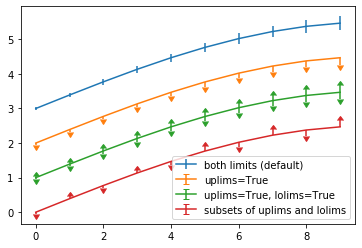
\includegraphics{./example_python_files/figure-pdf/cell-3-output-1.png}

\appendix
\addcontentsline{toc}{part}{Appendices}

\hypertarget{how-to-add-to-the-book}{%
\chapter*{How to add to the book}\label{how-to-add-to-the-book}}
\addcontentsline{toc}{chapter}{How to add to the book}

\hypertarget{set-up-quarto}{%
\section*{Set up Quarto}\label{set-up-quarto}}
\addcontentsline{toc}{section}{Set up Quarto}

This book is made with \href{https://quarto.org/}{Quarto}. Please see
the \href{https://quarto.org/docs/get-started/}{Get Started} chapter of
the Quarto documentation to learn how to install and run Quarto in your
IDE.

\hypertarget{add-to-book}{%
\section*{Add to book}\label{add-to-book}}
\addcontentsline{toc}{section}{Add to book}

Once you have everything set up, forked the repo, and cloned to your
computer, you can add a new chapter to the book.

Create a new file in the repository folder. For example, to create a new
file called \texttt{01\_exercises.qmd}, navigate to the folder then
create one using \texttt{touch\ 01\_exercises.qmd}. If you are using
VSCode, you can use the Quarto plug-in. You can use \texttt{.qmd} or
\texttt{.ipynb} files that run computations if you would like, or just
plain \texttt{.md} files. Check out the files under Examples to see the
various options.

Write in what you would like in the file.

Then, in the \texttt{\_quarto.yml} file, under \texttt{chapters}, add a
part with your chapter. The file listed after \texttt{part} is the first
page of chapter; the ones under \texttt{chapters} will be subpages.

\begin{Shaded}
\begin{Highlighting}[]
\AttributeTok{  }\KeywordTok{{-}}\AttributeTok{ }\FunctionTok{part}\KeywordTok{:}\AttributeTok{ 01\_main.qmd}
\AttributeTok{      }\FunctionTok{chapters}\KeywordTok{:}\AttributeTok{ }
\AttributeTok{      }\KeywordTok{{-}}\AttributeTok{ 01\_notes.qmd}
\AttributeTok{      }\KeywordTok{{-}}\AttributeTok{ 01\_video.qmd}
\AttributeTok{      }\KeywordTok{{-}}\AttributeTok{ 01\_exercises.qmd}
\end{Highlighting}
\end{Shaded}

\hypertarget{render-the-book}{%
\section*{Render the book}\label{render-the-book}}
\addcontentsline{toc}{section}{Render the book}

Once you have added and edited your files, don't forget to render the
book. Run this in the terminal:

\begin{Shaded}
\begin{Highlighting}[]
\ExtensionTok{quarto}\NormalTok{ render }\AttributeTok{{-}{-}to}\NormalTok{ html}
\end{Highlighting}
\end{Shaded}

\hypertarget{push-up-to-github}{%
\section*{Push up to GitHub}\label{push-up-to-github}}
\addcontentsline{toc}{section}{Push up to GitHub}

Push your changes to your forked repo and then create a pull request for
the R4DS admins to merge your changes.

\begin{Shaded}
\begin{Highlighting}[]
\FunctionTok{git}\NormalTok{ add .}
\FunctionTok{git}\NormalTok{ commit }\AttributeTok{{-}m} \StringTok{"Message here"}
\FunctionTok{git}\NormalTok{ push}
\end{Highlighting}
\end{Shaded}


\end{document}
